\chapter{Цели и задачи работы}
\textbf{Цель работы} --- аппроксимация неизвестной зависимости параболой.
\textbf{Содержание работы:}
\begin{enumerate}
\item Для выборки $(y_i, t_i),  = \overline{1; n}$, реализовать в виде программы на ЭВМ:
\begin{enumerate}
\item вычисление МНК-оценки вектора $\theta = (\theta_0, \theta_1, \theta_2)$ (в программе обозначатеся как theta) параметров модели $y = \theta_0 + \theta_1 t + \theta_2 t^2$;
\item вычисление среднеквадратичного отклонения $\delta = \sqrt{\sum\limits^n_{i=1} (y_i - y(t_i))^2}$ (в программе обозначается как delta) полученной модели от результатов наблюдений;
\item построение на одном графике системы точек $(y_i, t_i), i = \overline{1;n}$ и графика функции $y = y(t), t \in [t_{(1)}; t_{(n)}]$ (для полученной оценки вектора $\theta$).
\end{enumerate}
\item провести необходимые вычисления и построить соответствующие графики для выборки из индивидуального варианта.
\end{enumerate}

\chapter{Теоретическая часть}
\section{Постановка задачи аппроксимации неизвестной зависимости по результатам наблюдений}
Пусть имеются результаты n наблюдений:\\
\begin{equation}
\begin{cases}
y_1 = \Phi(x_1) + \xi_1\\
...\\
y_n = \Phi(x_n) + \xi_n\\
\end{cases}
\end{equation}
где:\\
$y_1, ..., y_n$ - n реализаций Y;\\
$\xi_1, ..., \xi_n$ - n реализаций $\xi$;\\
$x_1, ..., x_n$ - известные значения.\\

Задача аппроксимации - требуется на основе этих данных подобрать функцию $\hat\Phi$ так, чтобы она наилучшим образом аппроксимировала неизвестную функцию $\Phi$.

\section{Понятие МНК-оценки параметров линейной модели}
В качестве функции $\hat\Phi$ используется функция следующего вида:\\
$\hat\Phi(x) = \theta_1 \psi_1(x) + ... + \theta_p \psi_p (x)$, где: $\psi_1 ... \psi_p$ - известные функции.

Параметры $\theta_1, ..., \theta_p$ подбираются таким образом, чтобы $\hat\Phi(x)$ наилучшим образом аппроксимировала $\Phi(x)$. С учётом предположения о виде функции $\hat\Phi$ результат наблюдений можно записать в виде:\\
$y_i = \theta_1 \psi_1(x_i) + ... + \theta_p \psi_p (x_i) + \xi_i, i = \overline(1; n)$\\
В матричном виде:\\
$\overrightarrow{y} = \varepsilon \overrightarrow{\theta} + \overrightarrow{\xi}$, где:\\

\begin{align*}
    & \overrightarrow{y} = \begin{pmatrix} 
        y_1    \\ 
        y_2    \\ 
        \vdots \\ 
        y_n 
    \end{pmatrix},
    & \Psi &= \begin{pmatrix}
        \psi_1(x_1) & \psi_2(x_1) & \cdots & \psi_p(x_1) \\
        \psi_1(x_2) & \psi_2(x_2) & \cdots & \psi_p(x_2) \\
        \vdots      & \vdots      & \ddots & \vdots      \\
        \psi_1(x_n) & \psi_2(x_n) & \cdots & \psi_p(x_n)
    \end{pmatrix},
    & \vec{\theta} &= \begin{pmatrix}
        \theta_1 \\
        \theta_2 \\ 
        \vdots   \\ 
        \theta_p
    \end{pmatrix},
    & \overrightarrow{\varepsilon} = \begin{pmatrix} 
        \varepsilon_1 \\
        \varepsilon_2 \\ 
        \vdots        \\ 
        \varepsilon_n
    \end{pmatrix}.
\end{align*} 

Задача заключается в подборе $\overrightarrow{\theta}$. При этом предполагается, что систематические ошибки отсутствуют ($M\xi = 0$) и $\xi \tilde N(0, \sigma^2)$.

Оценка $\overrightarrow{\theta}$ вектора $\overrightarrow\theta$ называется оценкой, полученный по методу МНК (метода наименьших квадратов), если $\overrightarrow\theta$ минимизирует функцию $S(\overrightarrow\theta)=|y - \varepsilon \overrightarrow\theta|^2$.

\section{Формулы для вычисления МНК-оценки параметров модели}

Для данной работы МНК-оценка вектора $\vec\theta$ имеет вид:\\
$\hat\vec\theta = (\varepsilon^T \varepsilon)^{-1} \cdot \varepsilon^T \vec{y}$

Так как $y = \theta_0 + \theta_1 t + \theta_2 t^2$, то:\\

$
    \Psi = \begin{pmatrix}
        1      & t_1    & t_1^2  \\
        1      & t_2    & t_2^2  \\
        \vdots & \vdots & \vdots \\
        1      & t_n    & t_n^2
    \end{pmatrix}
$\\

Среднеквадратическое отклонение полученной модели от результатов наблюдений будет вычисляться как:\\
$\delta = \sqrt{\sum\limits^n_{i=1}(y_i - y(t_i)^2)^2},$ где:\\
$y_i$ - реальное значение\\
$y(t_i)$ - предсказанное значение.

\chapter{Практическая часть}

\section{Результаты работы для выборки по варианту}
\begin{lstlisting}
Lab 3
theta =

  -2.2797
   3.9880
   9.0604

delta = 43.398
\end{lstlisting}

\begin{figure}[H]
	\center{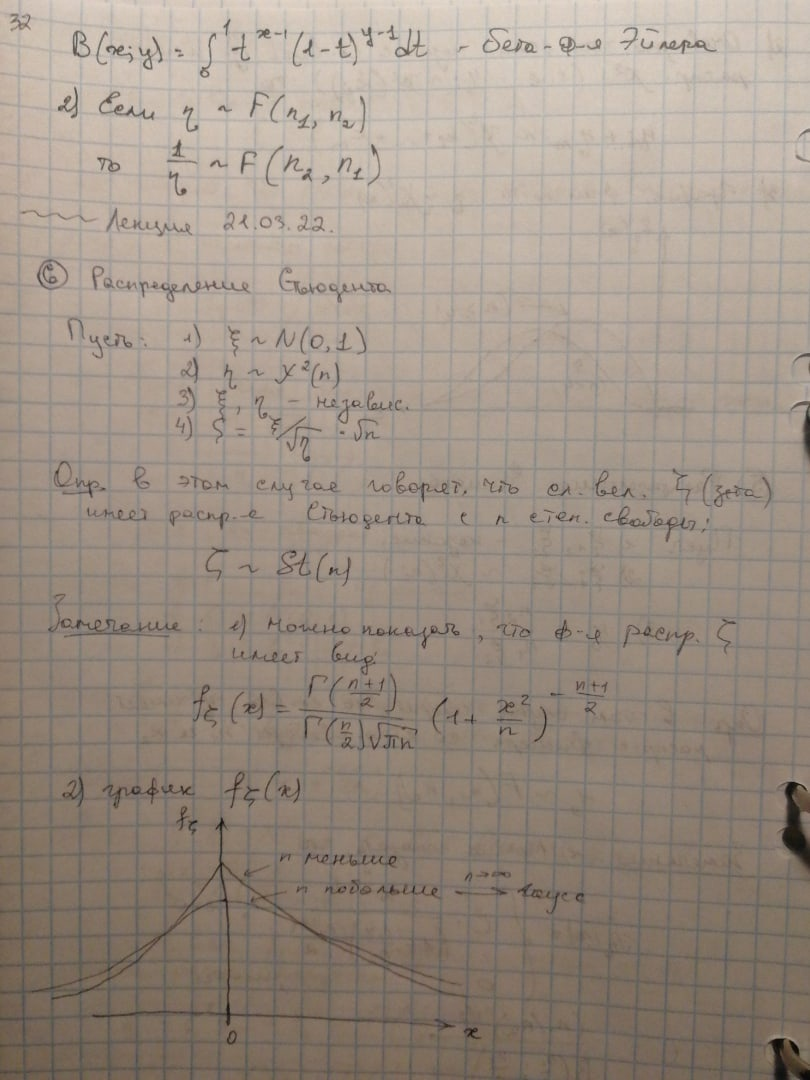
\includegraphics[scale=1.3]{1}}
\end{figure}
\newpage

\section{Листинг программы}
\begin{lstlisting}
disp("Lab 3")
pkg load statistics

T=[-5.00,-4.80,-4.60,-4.40,-4.20,-4.00,-3.80,-3.60,-3.40,-3.20,-3.00,
-2.80,-2.60,-2.40,-2.20,-2.00,-1.80,-1.60,-1.40,-1.20,-1.00,-0.80,-0.60,
-0.40,-0.20,0.00,0.20,0.40,0.60,0.80,1.00,1.20,1.40,1.60,1.80,2.00,2.20,
2.40,2.60,2.80,3.00,3.20,3.40,3.60,3.80,4.00,4.20,4.40,4.60,4.80,5.00,
5.20,5.40,5.60,5.80,6.00,6.20,6.40,6.60,6.80,7.00];

Y=[197.43,183.86,178.27,161.81,140.28,118.66,117.68,103.34,88.89,
72.14,67.75,57.64,51.03,39.72,29.88,31.69,17.22,23.26,7.05,4.66,-5.12,
0.40,7.94,2.95,-0.36,-7.17,-4.61,10.91,-5.12,13.11,7.01,19.83,19.63,30.48,
21.92,39.36,47.14,54.18,64.60,80.99,82.72,110.69,122.67,137.00,153.09,
145.66,170.25,197.83,214.42,222.67,251.72,256.63,280.05,302.21,323.86,
349.56,367.37,399.31,419.74,442.23,470.16];

function Psi = psiMat(T)
  n = numel(T);
  p = 3;
  Psi = zeros(n, p);
  for i = 1:n
    Psi(i, 1) = 1;
    Psi(i, 2) = T(i);
    Psi(i, 3) = T(i) * T(i);
  endfor
endfunction

function delta = calcDelta(y, y_new)
  n = numel(y);
  sum = 0;
  for i = 1:n
    sum = sum + (y(i) - y_new(i)) * (y(i) - y_new(i)); 
  endfor
  delta = sqrt(sum);
endfunction

psiMatrix = psiMat(T);
theta = (psiMatrix' * psiMatrix) \ (psiMatrix' * Y');
disp(theta);

n = numel(Y);
y = zeros(1, n);
for i =  1:n
  y(i) = theta(1) + theta(2) * T(i) + theta(3) * T(i) * T(i);
endfor

delta = calcDelta(Y, y);
delta

figure();
hold on;
plot(T, Y, 'b');
plot(T, y, 'r');
hold off;
\end{lstlisting}